\documentclass[aspectratio=169, 12pt]{beamer}
\usepackage{bbm}
\usepackage[utf8]{inputenc}
\usepackage[T2A]{fontenc}
\usepackage[english,russian]{babel}
\usepackage{amscd,amssymb}
\usepackage{amsfonts,amsmath,array}
\usepackage{sidecap}
\usepackage[T2A]{fontenc}
\usepackage[utf8]{inputenc}
\usepackage{graphicx}				% Вставка картинок правильная
\graphicspath{{pictures/}, {images/}, {}}
\DeclareGraphicsExtensions{.pdf,.png,.jpg}
\usepackage{pdfpages}
\usepackage{multicol}

% Для алгоритмов
\usepackage{algorithm}
\usepackage{algpseudocode}
% Цвета 
\usepackage{color}
\usepackage{colortbl}

% Создаем новую команду для assumptions
%----------------------------------------------------------------------------------------------------------
\newtheorem*{assumption*}{\assumptionnumber}
\providecommand{\assumptionnumber}{}
\makeatletter
\newenvironment{assumption}[2]
 {%
  \renewcommand{\assumptionnumber}{\textbf{Assumption} #1 ({#2})}%
  \begin{assumption*}%
  \protected@edef\@currentlabel{#1-#2}%
 }
 {%
  \end{assumption*}
 }

%beamer  theme's used to be here :)
%\usetheme{mipt_beamer}
\usetheme{boxes}

%----------------------------------------------------------------------------------------------------------
\title[\hbox to 56mm{Feature}]{Methods with preconditioning with weight decay regularization}
\author[M.\,K.~Kreinin]{Matvei Kreinin}
\institute{Moscow Institute of Physics and Technology}
\date{\footnotesize
\par\smallskip\emph{Course:} My first scientific paper\par (Strijov's practice)/Group 003 %821, 813
\par\smallskip\emph{Expert:} A. Beznosikov
\par\bigskip\small 2023}

\begin{document}
\maketitle
\begin{frame}{Goal of researches}
    \textbf{Goal objectives:} create new method of optimization and investigate theory and practical convergence of algorithms.

    \textbf{Problem:} 
    \begin{itemize}
        \item Prove the convergence of the method AdamW and OASIS.
        \item Research the  convergence on practical tasks.
        \item Create and investigate new optimization algorithm 
        \item Compare it with the others
    \end{itemize}
\end{frame}

\begin{frame}{Notation}
\begin{itemize}
    \item Minimization problem:
    $$ \min_{x \in \mathbb{R}^d} f(x) $$
    
    \item Objective function $f(x)$
    
    \item $r(x)$ -- regularization function, $r(x) = \frac{\lambda}{2} ||x||_2^2$

    
    \item Objective function for AdamL2 method -- $f(x) + r(x)$, where $r(x) = \frac{\lambda}{2} ||x||_2^2$
    
    \item $D_t$ -- pseudo hessian on t-step, (AdamW: diagonal matrix of squares of gradients, OASIS: calculated only diagonal elements with Rademacher distribution)

    \item New regularization function $\tilde{r}(x) :$ $\nabla \tilde{r}(x) = D_t \nabla r(x)$

    \item New objective function $\tilde{F}(x) = f(x) + \tilde{r}(x) $
    
\end{itemize}
\end{frame}

\begin{frame}{Assumptions}
    \begin{assumption}{1}{Convex}
	The function f is convex, i.e. $\forall x, y \in \mathbb{R}^d$
	\begin{equation*}
		f(y) \geq f(x) + \langle \nabla f(x), y-x \rangle
	\end{equation*}
\end{assumption}

\begin{assumption}{2}{L-smoothness}
	The gradients of F are L-Lipschitz continuous $\forall w \in \mathbb{R}^d$, i.e. there exists a constant $L > 0$ such that $\forall x, y \in \mathbb{R}^d$,
	\begin{equation*}
		f(x) \leq f(y) + \langle \nabla f(y), x-y \rangle + \frac{L}{2} ||x - y||^2
	\end{equation*}
\end{assumption}
\end{frame}

\begin{frame}{Assumptions}
    \begin{assumption}{3}{$\mu$ - strongly convex}
	The function f is $\mu$-strongly convex, i.e., there exists a constant $\mu > 0$ such that $\forall x, y \in \mathbb{R}^d$
	\begin{equation*}
		f(x) \geq f(y) + \langle f(y), x-y \rangle +\frac{\mu}{2} ||x - y||^2
	\end{equation*}
\end{assumption}

\begin{assumption}{4}{PL--condition}
	If there exists $\mu > 0$, such that $||\nabla f(w) || \geq 2 \mu (f(w) - f^*)$, $\forall w \in \mathbb{R}^d$
\end{assumption}

\begin{assumption}{5}{l-smoothness}
	The gradient of r is l-Lipschitz continuous $\forall w \in \mathbb{R}^d$, i.e. there exists a constant $l > 0$ such that $\forall x, y \in \mathbb{R}^d$,
	\begin{equation*}
		r(x) \leq r(y) + \langle \nabla r(y), x-y \rangle + \frac{l}{2} ||x - y||^2
	\end{equation*}
\end{assumption}
\end{frame}

\begin{frame}{Algorithms}
    \begin{columns}
		\begin{column}{0.5\textwidth}
			\begin{algorithm}[H]
            
            \caption{General scheme for preconditions methods}\label{alg:genalg}
    
            \begin{algorithmic}
            \small{
            \Require{$\eta, \epsilon, f, r$}
            
            \While {$w$ not converged}
            \State $t = t+1$
            \State $g_t = \nabla f_t(w_{t-1})$
            \State $D_t =$ \textcolor{red}{diag($\sqrt{g_t \odot g_t} + \varepsilon$)} \footnote[1]{\textcolor{red}{red - AdamW}}
            \State $D_t$ = \textcolor{cyan}{$\mathbb{E}[z^T \nabla^2f(w_{t-1}) z]$} \footnote[2]{\textcolor{cyan}{cyan - OASIS}, where $z$ in Rademacher distribution}
            \State $w_t = w_{t-1} - \eta \cdot g_t D_t^{-1}$    
            \EndWhile
            }
\end{algorithmic}
\end{algorithm}
		\end{column}
		
		\begin{column}{0.55\textwidth} 
	     	
            \begin{algorithm}[H]
            
            \caption{Adam($\lambda$)}\label{alg:Adam}
    
            \begin{algorithmic}
            \small{
            \Require{$\eta, \beta_1, \beta_2, \epsilon, f, r$}
            %\State $m_0 = 0$ -- 1-st moment vector
            %\State$v_0 = 0$ -- 2-nd moment vector
            \While {$\theta$ not converged}
            \State $t = t+1$
            \State $g_t = \nabla f(w_{t-1})$ + \textcolor{blue}{$\nabla r(w_{t-1})$}\footnote{\textcolor{blue}{blue -- AdamL2}} 
            \State $m_t = \beta_1 \cdot m_{t-1} + (1 - \beta_1) \cdot g_t$
            \State $v_t = \beta_2 \cdot v_{t-1} + (1 - \beta_2) \cdot g_t^2$
            \State $\hat{m_t} = \frac{m_t}{1-\beta_1^t}$ + \textcolor{yellow}{$\nabla r(w_{t-1})$} \footnote{\textcolor{yellow}{yellow -- MyAdamW}}
            \State $\hat{v_t} = \frac{v_t}{1-\beta_2^t}$ 
            \State $w_t = w_{t-1} - \eta \cdot \frac{\hat{m_t}}{\sqrt{v_t} + \epsilon}$    - \textcolor{red}{$\eta \nabla r(w_{t-1})$ } \footnote{\textcolor{red}{red - AdamW}}
            \EndWhile
            }
\end{algorithmic}
\end{algorithm}


		\end{column}
	\end{columns}
\end{frame}

\begin{frame}{Theorem №1}
\begin{theorem}[1]
Suppose the Assumption 1, 2, 5 and let $\varepsilon > 0$ and let the step-size satisfy
\begin{equation*}
    \eta < \frac{2 \alpha}{L + l \cdot \alpha} 
\end{equation*}
Then, the number of iterations performed by AdamW algorithm, starting from an initial point $w_0 \in \mathbb{R}^d$ with $\Delta_0 = \tilde{F}(w_0) - \tilde{F}^*$, required to obtain and $\varepsilon$-approximate solution of the convex problem (link here to problem 1) can be bounded by
\begin{equation*}
      T = \mathcal{O}\left( \frac{2\Delta_0 \Gamma \alpha } {(2\alpha - \tilde{L}\eta) \eta \varepsilon} \right)
\end{equation*}

\end{theorem}
\end{frame}
\begin{frame}{Proof Theorem №1 (1/4)}
    
Let's write first assumption for step t and $t+1$:

\begin{equation*}
    f(w_{t+1}) \leq f(w_t) + \langle \nabla f(w_t), w_{t+1} - w_t \rangle + \frac{L}{2}||w_{t+1} - w_t ||^2,
\end{equation*}
Okay, by definition for our algorithm we have:

\begin{equation*}
w_{t+1} - w_t = -\eta D_t^{-1} \nabla f(w_t) - \eta \nabla r(w_t),
\end{equation*}
and 

\begin{equation*}
\nabla f(w_t) = \frac{1}{\eta} D^t(w_t - w_{t+1}) - D^t \nabla r(w_t),
\end{equation*}

\end{frame}

\begin{frame}{Proof Theorem №1 (2/4)}
    Okay, now let's replace $\nabla f(w_t)$ and $I \leq \frac{D_t}{\alpha}$
\begin{equation*}
    f(w_{t+1}) \leq f(w_t) + \langle \frac{1}{\eta}D_t(w_t - w_{t+1}) - D_t\nabla r(w_t), w_{t+1} - w_t \rangle + \frac{L}{2 \alpha} ||w_{t+1} - w_t||_{D_t}^2,
\end{equation*}

\begin{equation*}
    f(w_{t+1}) \leq f(w_t) + \left(\frac{L}{2 \alpha} - \frac{1}{\eta} \right) ||w_{t+1} - w_t||_{D_t}^2 - \langle D_t \nabla r(w_t), w_{t+1} - w_t \rangle,
\end{equation*}

Lets define new variable $\tilde{r} : \nabla \tilde{r} = D_t \nabla r(w_t)$. Then rewrite step using the variable and 5-th assumption.
\begin{equation*}
    \tilde{r}(w_{t+1}) \leq \tilde{r}(w_t) + \langle \tilde{r}(w_t), w_{t+1} - w_t \rangle + \frac{l}{2} (w_{t+1} - w_t)^T D_t (w_{t+1} - w_t),
\end{equation*}
\end{frame}

\begin{frame}{Proof Theorem №1 (3/4)}
    \begin{equation*}
    f(w_{t+1}) \leq f(w_t) + \left( \frac{L}{2\alpha} - \frac{1}{\eta} \right) ||w_{t+1} - w_t||_{D_t}^2 + \tilde{r}(w_t) - \tilde{r}(w_{t+1}) + \frac{l}{2}||w_{t+1}-w_t||_{D_t}^2,
\end{equation*}

$\tilde{F}(w) = f(w) + \tilde{r}(w)$, $F(w) = f(w) + r(w)$, ($\tilde{L}=L + l \alpha$), we get:

\begin{equation*}
    \tilde{F}(w_{t+1}) \leq \tilde{F}(w_t) + \left( \frac{\tilde{L}}{2\alpha} - \frac{1}{\eta}  \right) ||w_{t+1} - w_t||_{D_t}^2,
\end{equation*}


\begin{equation*}
    \left(\frac{1}{\eta} - \frac{\tilde{L}}{2\alpha}   \right) ||w_{t+1} - w_t||_{D_t}^2 \leq \tilde{F}(w_t) - \tilde{F}(w_{t+1})
\end{equation*}
\end{frame}

\begin{frame}{Proof Theorem №1 (4/4)}
\begin{eqnarray*}
&& \frac{\eta^2  (T+1)}{\Gamma}\left(\frac{1}{\eta} - \frac{\tilde{L}}{2\alpha}   \right)\cdot\min_{k = 0, T} ||\nabla f(w_t) + \nabla \tilde{r}(w_t)||^2 \leq
\notag\\&\leq&
\frac{\eta^2}{\Gamma}\left(\frac{1}{\eta} - \frac{\tilde{L}}{2\alpha}   \right)\cdot\sum\limits_{t = 0}^T ||\nabla f(w_t) + \nabla \tilde{r}(w_t)||^2 \leq \tilde{F}(w_0) - \tilde{F}(w_*),    
\end{eqnarray*}

\begin{equation*}
    \min_{t = 0, T} ||\nabla f(w_t) + \nabla \tilde{r}(w_t)||^2 \leq \frac{(\tilde{F}(w_0) - \tilde{F}(w_*))\Gamma}{(\frac{1}{\eta} - \frac{\tilde{L}}{2\alpha}) \eta^2 (T+1)} = \varepsilon,
\end{equation*}

\begin{equation*}
    T + 1 \geq \frac{\Delta_0 \Gamma}{(\frac{1}{\eta} - \frac{\tilde{L}}{2\alpha}) \eta^2 \varepsilon}
\end{equation*}
    Then:
\begin{equation*}
      T = \mathcal{O}\left( \frac{2\Delta_0 \Gamma \alpha } {(2\alpha - \tilde{L}\eta) \eta \varepsilon} \right)
\end{equation*}
\end{frame}

\begin{frame}{Theorem №2}
    \begin{theorem}
    Suppose the Assumption 1, 2, 4, 5 and let $\varepsilon > 0$ and let the step-size satisfy
    \begin{equation*}
        \eta \leq \frac{2 \alpha}{\tilde{L}}
    \end{equation*}
    Then, the number of iterations performed by AdamW algorithm, starting from an initial point $w_0 \in \mathbb{R}^d$ with $\Delta_0 = \tilde{F}(w_0) - \tilde{F}^*$, required to obtain and $\varepsilon$-approximate solution of the convex problem (link here to problem 1) can be bounded by
    \begin{equation*}
        T =  \mathcal{O}\left( \frac{\ln \frac{\Delta_0}{\epsilon}}{2 \mu \eta^2(\frac{1}{\eta} - \frac{\tilde{L}}{2 \alpha})} \right)
    \end{equation*}
\end{theorem}
\end{frame}

\begin{frame}{Proof Theorem №2}
        Assume 
    \begin{equation*}
    \nabla \tilde{F} = \nabla f + \nabla \tilde{r}    
    \end{equation*}
    
    \begin{equation*}
    L + ||D_t||l = \tilde{L}        
    \end{equation*}
    
    \begin{equation*}
    w_{t+1} - w_t = -\eta D_t^{-1} \nabla r(w_t) - \eta \nabla r(w_t) = -\eta D_t^{-1} (\nabla f + \nabla \tilde{r})(w_t) = -\eta D_t^{-1} \nabla \tilde{F}(w_t)    
    \end{equation*}
    
    Then we write $\tilde{L}$-smoothness for $\tilde{F}$ 
    \begin{equation*}
        \tilde{F}(w_{t+1}) - \tilde{F}(w_t) \leq  \langle \nabla \tilde{F}(w_t), w_{t+1} - w_t \rangle + \frac{\tilde{L}}{2} ||w_{t+1} - w_t||^2
    \end{equation*}

    
\end{frame}

\begin{frame}{Proof Theorem №2}
    \begin{eqnarray*}
    &&
    \tilde{F}(w_{t+1}) - \tilde{F}(w_t) \leq - \langle \frac{1}{\eta} D_t(w_{t+1} - w_t), w_{t+1} - w_t \rangle + \frac{\tilde{L}}{2} ||w_{t+1} - w_t||^2 = 
    \notag\\&\ = &
    (\frac{\tilde{L}}{2 \alpha} - \frac{1}{\eta}) ||w_{t+1} - w_t||^2_{D_t} = (\frac{\tilde{L}}{2 \alpha} - \frac{1}{\eta}) ||-\eta D_t^{-1} \nabla \tilde{F}(w_t)||_{D_t}^2 \leq
    \notag\\&\ \leq &  (\frac{\tilde{L}}{2 \alpha} - \frac{1}{\eta}) \eta^2 ||\nabla \tilde{F}(w_t)||^2_{D_t^{-1}}
    \end{eqnarray*}
    
    Then we use PL-condition for the function $\tilde{F}$:
    \begin{equation*}
        ||\nabla \tilde{F}(w_t)||_{D_t^{-1}}^2 \geq 2 \mu (\tilde{F}(w_t) - \tilde{F}^*)
    \end{equation*}
\end{frame}

\begin{frame}{Proof Theorem №2}
    \begin{eqnarray*}
&& \tilde{F}(w_{t}) -  F^* \ge \tilde{F}(w_{t+1}) - \tilde{F}^* + (\frac{1}{\eta} - \frac{\tilde{L}}{2 \alpha}) \eta^2 2 \mu (\tilde{F}(w_t) - \tilde{F}^*)=
\notag\\&\ = & \left( 1 +  2 \mu \eta^2(\frac{1}{\eta} - \frac{\tilde{L}}{2 \alpha}) \right) (\tilde{F}(w_{t+1}) - \tilde{F}^*),    
\end{eqnarray*}
    
    \begin{equation*}
    \epsilon \ge \Delta_0 \left( 1 +  2 \mu \eta^2(\frac{1}{\eta} - \frac{\tilde{L}}{2 \alpha}) \right)^{-T} \ge (\tilde{F}(w_{T}) - \tilde{F}^*)        
    \end{equation*}

    \begin{equation*}
    T = \frac{\ln \frac{\Delta_0}{\epsilon}}{\ln(1 + 2 \mu \eta^2(\frac{1}{\eta} - \frac{\tilde{L}}{2 \alpha}))} \approx \frac{\ln \frac{\Delta_0}{\epsilon}}{2 \mu \eta^2(\frac{1}{\eta} - \frac{\tilde{L}}{2 \alpha})}        
    \end{equation*}
    Then:
    \begin{equation*}
    T =  \mathcal{O}\left( \frac{\ln \frac{\Delta_0}{\epsilon}}{2 \mu \eta^2(\frac{1}{\eta} - \frac{\tilde{L}}{2 \alpha})} \right)
    \end{equation*}
\end{frame}

\begin{frame}{Experiments}
    Experimental conditions
        \begin{itemize}
            \item Model: ResNet18 (100 epoch),
            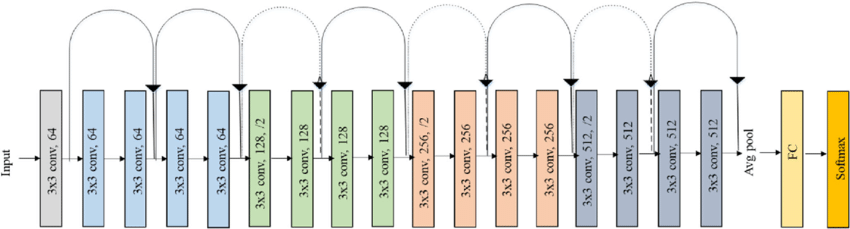
\includegraphics[scale=0.3]{resnet18.png}
            
            \item CosineAnnealingLR scheduler: $\eta_t = \eta_{min} + \frac{1}{2} \left( \eta_{min} + \eta_{max} \right) \left(1 + cos\left(\frac{T_{cur}}{T_{max} \pi} \right) \right)$
            \item Grid of learning rates = [0.01, 0.005, 0.0005], 
            weight decays = [0.005, 0.0005, 0.00005]
            \item Data set: CIFAR10. The CIFAR-10 dataset consists of 60000 32x32 colour images in 10 classes, with 6000 images per class. There are 50000 training images and 10000 test images. 
        \end{itemize}
     
\end{frame}

\begin{frame}{Experiment}              
    Training loss (epoch)
\begin{center}
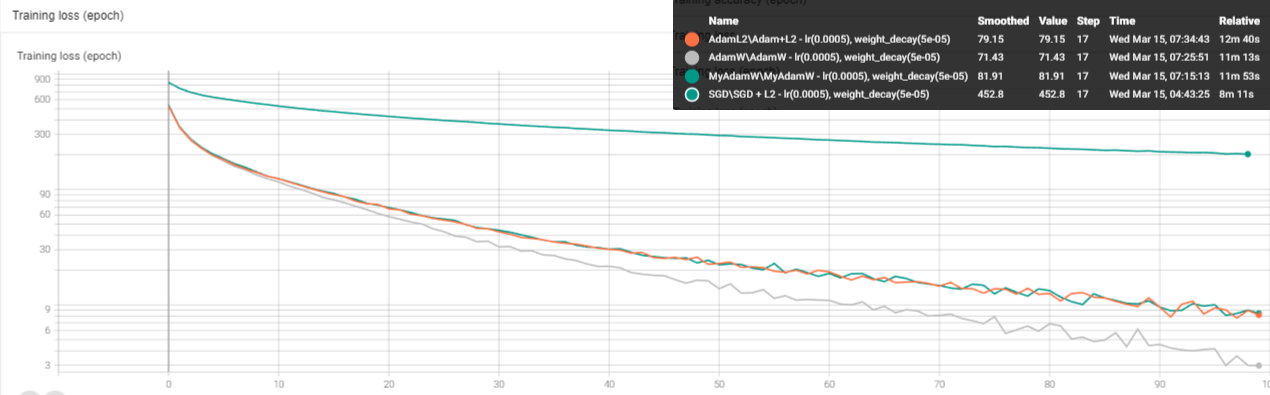
\includegraphics[width=0.7\textwidth, height=0.3\textheight]{training_loss.png}
\end{center}
    Testing accuracy (loss)
\begin{center}
    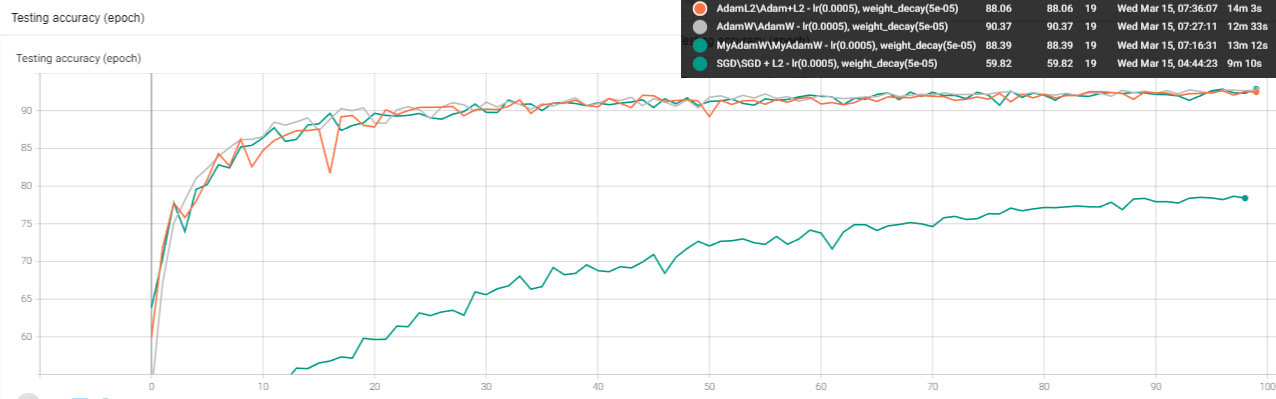
\includegraphics[width=0.7\textwidth, height=0.3\textheight]{testing_accuracy.png}
\end{center}
\end{frame}

\if 0
\begin{frame}
	\frametitle{Methods with preconditioning with weight decay regularization}

	\begin{columns}
		\begin{column}{0.5\textwidth}
			\begin{block}{Assumptions}
				\begin{itemize}
				
					\item The function f is convex, i.e. $\forall y, x \in \mathbb{R}^d$
	\begin{equation*}
		f(y) \geq f(x) + \langle \nabla f(x), y-x \rangle
	\end{equation*}
                        \item The gradients of F are L-Lipschitz continuous $\forall w \in \mathbb{R}^d$, i.e. there exists a constant $L > 0$ such that $\forall x, y \in \mathbb{R}^d$,
	\begin{equation*}
		f(x) \leq f(y) + \langle \nabla f(y), x-y \rangle + \frac{L}{2} ||x - y||^2
	\end{equation*}
                        \item The function f is twice continuously differentiable.
                       
				\end{itemize}
			\end{block}		
		\end{column}
		
		\begin{column}{0.55\textwidth} 
	     	\begin{block}{Experimental conditions}
            \begin{algorithm}[H]
            
            \caption{MyAdamW($\lambda$)}\label{alg:Adam}
    
            \begin{algorithmic}
            \small{
            \Require{$\alpha, \beta_1, \beta_2, \epsilon, f, r$}
            %\State $m_0 = 0$ -- 1-st moment vector
            %\State$v_0 = 0$ -- 2-nd moment vector
            \While {$\theta$ not converged}
            \State $t = t+1$
            \State $g_t = \nabla_{\theta} f_t(\theta_{t-1})$
            \State $m_t = \beta_1 \cdot m_{t-1} + (1 - \beta_1) \cdot g_t$
            \State $v_t = \beta_2 \cdot v_{t-1} + (1 - \beta_2) \cdot g_t^2$
            \State $\hat{m_t} = \frac{m_t}{1-\beta_1^t}$
            \State $\hat{v_t} = \frac{v_t}{1-\beta_2^t} +\nabla_{\theta} r(\theta)$
            \State $\theta_t = \theta_{t-1} - \alpha \cdot \frac{\hat{m_t}}{\sqrt{v_t} + \epsilon}$    \EndWhile
            }
\end{algorithmic}
\end{algorithm}

            \end{block}     

		\end{column}
	\end{columns}


\begin{columns}

	\begin{column}{0.5\textwidth}
		\begin{block}{Assumptions}
    \begin{itemize}
			 \item The gradient of r is l-Lipschitz continuous $\forall w \in \mathbb{R}^d$, i.e. there exists a constant $l > 0$ such that $\forall x, y \in \mathbb{R}^d$,
	\begin{equation*}
		r(x) \leq r(y) + \langle \nabla r(y), x-y \rangle + \frac{l}{2} ||x - y||^2
	\end{equation*}
			\end{itemize}
		\end{block}	
	

	\end{column}
	
	\begin{column}{0.57\textwidth}  
             \begin{block}{Theorem}
                    Original problem: $\min f(w)$
                    
                    $\tilde{F}(w) = f(w) + \tilde{r}(w)$, $\nabla \tilde{r}(w) = D_t \nabla r(w)$, $\alpha \cdot I \leq D_t \leq \Gamma \cdot I$
                    \begin{equation*}
     ||\nabla f(w_N) + \nabla \tilde{r}(w_N)||^2 \leq \dfrac{(\tilde{F}(w_0) - \tilde{F}(w_*))\Gamma}{(\frac{1}{\eta} - \frac{L + l\cdot \alpha}{2\alpha}) \eta^2 (N+1)}     
\end{equation*}
                  \end{block}		

	\end{column}
\end{columns}
\end{frame}
\fi
\end{document}